
\documentclass[10pt,twocolumn,letterpaper]{article}

\usepackage[pagenumbers]{cvpr} %
\usepackage{multirow}
\usepackage{multicol}
\usepackage{pgfplots}
\usepackage{svg}
\usepackage{tikz}
\usepackage{xcolor}
\usepackage{overpic}
\usetikzlibrary{calc,patterns,angles,quotes}
\usepackage{pgfplots,gincltex}
\pgfplotsset{compat=1.18}
\usepgfplotslibrary{colormaps}
\usepackage{tikz-3dplot}
\pgfplotsset{compat=newest}
\newcommand{\CG}{\mathcal{G}\xspace}
\newcommand{\CV}{\mathcal{V}\xspace}
\newcommand{\CE}{\mathcal{E}\xspace}
\newcommand{\CA}{\mathcal{A}\xspace}
\newcommand{\CF}{\mathcal{F}\xspace}
\newcommand{\CR}{\mathcal{R}\xspace}
\newcommand{\CB}{\mathcal{B}\xspace}
\newcommand{\CX}{\mathcal{X}\xspace}
\newcommand{\CK}{\mathcal{K}\xspace}
\newcommand{\CM}{\mathcal{M}\xspace}
\newcommand{\CC}{\mathcal{C}\xspace}
\newcommand{\CL}{\mathcal{L}\xspace}
\newcommand{\CI}{\mathcal{I}\xspace}
\newcommand{\CQ}{\mathcal{Q}\xspace}
\newcommand{\CO}{\mathcal{O}\xspace}
\newcommand{\CP}{\mathcal{P}\xspace}
\newcommand{\CS}{\mathcal{S}\xspace}
\newcommand{\CT}{\mathcal{T}\xspace}
\newcommand{\CJ}{\mathcal{J}\xspace}
\usepackage[para]{footmisc}
\usepackage{subfig}
% \usepackage{subcaption}
% \usepackage{array}
% \usepackage{colortbl}



\definecolor{cvprblue}{rgb}{0.21,0.49,0.74}
\definecolor{lightboldcolor}{gray}{0.6}
\usepackage[pagebackref,breaklinks,colorlinks,allcolors=cvprblue]{hyperref}

\newcommand{\ZL}[1]{{ \color{magenta}{ ZL: #1 }}}
\newcommand{\HZ}[1]{{ \color{cyan}{HZ: #1}}}
\newcommand{\lightbold}[1]{\textbf{\textcolor{lightboldcolor}{#1}}}


\def\paperID{12874} %
\def\confName{CVPR}
\def\confYear{2025}

\title{Laplace-Beltrami Operator for Gaussian Splatting}
\author{Hongyu Zhou$^{1,2}$ \qquad\qquad Zorah Lähner$^{1,2}$ \\
\ \\
$^1$University of Bonn \qquad \qquad $^2$Lamarr Institute\\
{\tt\small hzhou,laehner@uni-bonn.de}
}

\begin{document}

\twocolumn[{%
\renewcommand\twocolumn[1][]{#1}%
\maketitle
\begin{center}
    \centering
    \captionsetup{type=figure}
    \includegraphics[width=1.0\textwidth,height=4.6cm]{figures/teaser.png}
    \captionof{figure}{We introduce a novel method to accurately compute the Laplace-Beltrami operator directly on 3D Gaussian splats, leveraging both the center and the covariance information. The operator can be directly applied on 3D Gaussian splats, without the need for mesh extraction, for multiple applications such as surface smoothing, as shown above. We can transform the original scene (left) by computing the Laplace-Beltrami eigenfunctions (middle, both original and smoothed), leading to a smoothed scene of the 3D Gaussians splats (right), which presents transformation on the original rendering (left) and the computed Laplace-Beltrami eigenfunction (middle). %
\label{fig:teaser}}
\end{center}%
}]

\begin{abstract}

% Recent works to jointly reconstruct 3D human and object from a single RGB image, are mostly model-based, that fail to capture the fine details of the clothed human body and object surface. In this paper, we introduce ReCHOR, a novel, model-free, first-method to produce realistic clothed human-object reconstructions from a monocular view. This is extremely challenging due to human-object occlusions, diverse interactions and depth ambiguity, as it needs to infer both 3D spatial awareness and high resolution details. Our core idea is based on estimating neural implicit representations for human and object respectively by an attention-based neural implicit model that attends to pixel-aligned features from both the global human-object image for spatial awareness and  the local separate view of human and object images for high quality details. Additionally, the network is conditioned on semantic features from an initial estimated human-object pose prior and a generative diffusion model that inpaints occluded regions, thus enabling the retrieval of details from them.
% We also propose a synthetic dataset with rendered scenes of diverse, inter-occluded 3D human and object scans, to train our network. We evaluate our method on the synthetic and real world BEHAVE dataset. Our experiments show that our method outperforms the SOTA in achieving realistic clothed human-object reconstructions.
Recent approaches to jointly reconstruct 3D humans and objects from a single RGB image represent 3D shapes with template-based or coarse models, which fail to capture details of loose clothing on human bodies. In this paper, we introduce a novel implicit approach for jointly reconstructing realistic 3D clothed humans and objects from a monocular view. For the first time, we model both the human and the object with an implicit representation, allowing to capture more realistic details such as clothing. This task is extremely challenging due to human-object occlusions and the lack of 3D information in 2D images, often leading to poor detail reconstruction and depth ambiguity. To address these problems, we propose a novel attention-based neural implicit model that leverages image pixel alignment from both the input human-object image for a global understanding of the human-object scene and from local separate views of the human and object images to improve realism with, for example, clothing details. Additionally, the network is conditioned on semantic features derived from an estimated human-object pose prior, which provides 3D spatial information about the shared space of humans and objects. To handle human occlusion caused by objects, we use a generative diffusion model that inpaints the occluded regions, recovering otherwise lost details. For training and evaluation, we introduce a synthetic dataset featuring rendered scenes of inter-occluded 3D human scans and diverse objects. Extensive evaluation on both synthetic and real-world datasets demonstrates the superior quality of the proposed human-object reconstructions over competitive methods.
\end{abstract}    
\section{Introduction}
\label{sec:intro}
% Image editing methods in diffusion models depend on user-defined control directions - users can unlock their creativity using these methods by specifying the desired manipulation through prompts~\cite{gandikota2023concept}, reference images~\cite{ruiz2022dreambooth, kumari2022customdiffusion, gal2022image, chen2024trainingfreeregionalpromptingdiffusion}, or attribute vectors~\cite{parmar2023zero,hertz2022prompt}. In this work, we ask a fundamentally different question: \emph{Can we automatically discover the underlying visual structure of a concept within diffusion model's knowledge?} %Rather than requiring user-specified controls, we aim to decompose the model's internal knowledge into meaningful directions.

% This question touches on a fundamental limitation in how we interact with diffusion models. Current control methods ~\cite{zhang2023addingconditionalcontroltexttoimage, gandikota2023concept, ye2023ipadaptertextcompatibleimage,ye2023ipadaptertextcompatibleimage, hertz2024stylealignedimagegeneration, li2023photomaker, shi2024instantbooth, chen2024trainingfreeregionalpromptingdiffusion} require users to specify their desired manipulations in advance, limiting interactive creativity. This contrasts with natural human artistic workflows, where creators dynamically explore creative ideas while jointly refining them toward meaningful artistic outcomes~\cite{hoffmann2016modeling}. This synergy between specification and exploration is not new to generative models. Early GAN architectures naturally developed disentangled latent spaces that enabled continuous\cite{harkonen2020ganspace,radford2015unsupervised, wu2021stylespace, shen2020interfacegan}, compositional control over generated images. Users could explore these spaces to discover interesting variations that would be difficult to describe in words~\cite{wu2021stylespace}, then combine them to achieve their creative goals~\cite{grabe2022towards}. 


% While diffusion models have largely superseded GANs in conditional image synthesis~\cite{dhariwal2021diffusion},  their underlying structure remains less understood. Diffusion models achieve remarkable diversity through high-dimensional latents, unlike GANs' compact latent spaces.  With a single prompt, diffusion models can generate radically different variations through different random initializations of input noise. We ask - Is it possible to discover interpretable structure within this vast space of variations?

Text-to-image diffusion models are capable of generating remarkable visual variations from a single prompt through different random initializations. However, this vast creative potential remains largely opaque to users---while we can generate diverse images, we lack understanding of the underlying structure of these variations. This presents a fundamental challenge: how can we discover and expose the latent visual capabilities encoded within these models?

\let\thefootnote\relax \footnote{$^{*}$Correspondence to \texttt{gandikota.ro@northeastern.edu}}

The challenge touches on a key limitation in how we interact with diffusion models today. Current control methods require users to explicitly specify their desired edits in advance through prompts~\cite{gandikota2023concept}, reference images~\cite{zhang2023addingconditionalcontroltexttoimage, chen2024trainingfreeregionalpromptingdiffusion, ruiz2022dreambooth,kumari2022customdiffusion, Ryu_lora, hu2021lora}, or attribute vectors~\cite{ye2023ipadaptertextcompatibleimage, hertz2024stylealignedimagegeneration, li2023photomaker, shi2024instantbooth,parmar2023zero,hertz2022prompt}. That contrasts sharply with natural human creative workflows, where artists dynamically explore creative ideas and jointly refine them toward meaningful artistic outcomes~\cite{hoffmann2016modeling}. The need for pre-specified controls creates a barrier between users and the full creative potential of these models.

Interestingly, earlier generative models like GANs~\cite{gans,karras2019style,brock2018large} naturally developed more interpretable internal structures. Their compact latent spaces often exhibited emergent disentanglement~\cite{harkonen2020ganspace,radford2015unsupervised, wu2021stylespace, shen2020interfacegan}, enabling continuous and compositional control over generated images. Users could explore these spaces to discover interesting variations that would be difficult to describe in words~\cite{wu2021stylespace}, then combine them to achieve their creative goals~\cite{grabe2022towards}.

Diffusion models have largely superseded GANs in conditional image synthesis~\cite{dhariwal2021diffusion}, achieving greater diversity through much higher-dimensional latents. And yet an understanding of the underlying structure of these larger latent spaces has remained elusive. In this work, we ask a fundamental question: \emph{Can we automatically discover the visual structure within a diffusion model's knowledge of a concept?} Rather than requiring user-specified controls, we aim to decompose the model's internal representations into expressive directions that users can explore and combine.

To address these needs, we present \textbf{SliderSpace}, a framework that brings systematic explorability to diffusion models. Given just a text prompt, SliderSpace discovers a canonical set of meaningful, diverse, and controllable directions within the model's knowledge of that concept. Each direction is implemented as a low-rank adapter~\cite{hu2021lora} that can be scaled and composed with others, allowing users to explore and smoothly combine different aspects of variation, as shown in Figure~\ref{fig:intro}.

We ground SliderSpace discovery in three key requirements for meaningful decomposition of a diffusion model's visual manifold: 
\begin{enumerate}
    \item \textbf{Unsupervised Discovery:} The decomposition process should emerge from the intrinsic structure of the model's learned representation, rather than being guided by predefined attributes. This ensures we capture the true topology of the model's knowledge space rather than projecting our assumptions onto it.
    
    \item \textbf{Semantic Orthogonality:} Each discovered control must represent a distinct semantic direction. This is enforced in a semantic feature space, like CLIP, where every slider has an orthogonal effect in embeddings. This prevents discovering multiple controls that create similar semantic effects, making the system more efficient and easier.
    
    \item \textbf{Distribution Consistency:} Directions must induce consistent transformations across both random seeds and prompt variations. 
\end{enumerate}

These requirements naturally lead to our proposed framework, which we formalize in Section~\ref{sec:method}. As we show in our experiments, SliderSpace is architecture-agnostic, working with both conventional U-Net based models like Stable Diffusion~\cite{rombach2022high, rombach2022sd20, podell2023sdxl, turbo, dmd} and recent transformer-based architectures like Flux~\cite{flux}.

We demonstrate the expressiveness of SliderSpace through three applications: First, we show how SliderSpace can decompose high-level concepts into diverse and expressive components, revealing the natural axes of variation in the model's understanding. Second, we explore artistic style variation, where SliderSpace discovers directions that match or exceed the diversity of manually curated artist lists while being judged more useful by human evaluators. Finally, we show how SliderSpace can help reverse the mode collapse commonly observed in distilled diffusion models, restoring diversity while maintaining generation speed.

Beyond providing practical creative control, SliderSpace opens new avenues for understanding and utilizing the latent capabilities of diffusion models. By mapping these models' visual potential into intuitive, composable directions, we take a step toward making their creative possibilities more accessible and interpretable to users.

% Image editing methods in diffusion models unlock the creativity of users. In this work we ask an alternate question: \emph{Can we organize and expose what of the diffusion model is already capable of?}.
% Existing methods for controlling image generation typically require users to manually specify edit directions for desired changes. This process is time-consuming, requires technical expertise, and limits the spontaneity of the creative process. For instance, if a user wants to adjust the smile of a generated person, they must explicitly request this edit, often through imprecise prompt engineering or model fine-tuning. This approach of predefined controls or manual specifications restricts users from fully exploring the latent capabilities of the model. There may be interesting stylistic variations or attributes that the model can generate, but users have no easy way to discover or utilize these.

% Natural visual disentanglement was an emergent property in the latent space of Generative Adversarial Models (GANs) \cite{harkonen2020ganspace,radford2015unsupervised, wu2021stylespace, shen2020interfacegan}. In particular, it has been observed that StyleGAN~\cite{karras2019style} stylespace neurons offer detailed control over many meaningful aspects of images that would be difficult to describe in words~\cite{wu2021stylespace}. However, diffusion models do not share such a compact latent space~\cite{park2023unsupervised}; and efforts to uncover such a space in the semantic embeddings of the text conditioning have met with limited success \nik{Nick - is there a specific citation you were thinking about?}.

% In this work we introduce \textbf{SliderSpace}, which takes a step towards uncovering an analogous low dimensional representation of diffusion models' visual breadth; in essence treating the diffusion model as many generators sharing parameters, where a particular generator is defined by a specific prompt. For a given prompt we sample many random seeds (and optionally prompt expansions using an LLM), generate the corresponding images, and apply an off the shelf feature extractor (in this work CLIP, but our method can be applied to any differentiable feature extractor). We use PCA to analyze these features, and for each of the leading $k$ principal components we train a LoRA \cite{} which causes the diffusion model to produces images which increase the feature magnitude along that component when passed back through the same feature extractor. This leads to a 'Slider' for each principal component, because each LoRA can be scaled and applied to the original diffusion model, continuously varying those visual features in the generated results (as measured, in our case, by CLIP).

% There are many other works that enhance the controllability of diffusion models. One common approach is enabling users to add spatial constraints to a generation either manually, or via a reference image \cite{zhang2023addingconditionalcontroltexttoimage, chen2024trainingfreeregionalpromptingdiffusion}, a second is leveraging more abstract embeddings (e.g. identity, style) extracted from a reference image \cite{ye2023ipadaptertextcompatibleimage, hertz2024stylealignedimagegeneration, li2023photomaker, shi2024instantbooth}, a third is finetuning a foundation model to better generate a concept important to the user \cite{ruiz2022dreambooth, kumari2022customdiffusion, Ryu_lora, hu2021lora}, and a fourth (most relevant to this work) is finding low-rank adaptors of the model based on a prompt or small training set which can be scaled to provide continous control over one aspect of generated image (e.g. night vs day, basic vs luxury, etc.) \cite{gandikota2023concept}. SliderSpace is complementary to all of these methods and offers something distinct. All of the other methods we are aware require the user (and / or model designer) to know in advance what type of control they want. In contrast SliderSpace assists users in discovering and controlling hidden capabilities present in the diffusion model's distribution of possible generations.

%We propose that truly intuitive creative control in a text-to-image model should meet three key criteria: \emph{discoverability}, \emph{intuitiveness}, and \emph{specificity}. The model should reveal controllable attributes that may not be immediately obvious, offer controls that are easy to understand and manipulate, and ensure each control affects a distinct attribute of the generated image.

% We demonstrate the utility and power of SliderSpace using three applications built on top of SDXL-DMD \cite{dmd}, because its fast generation speed lends itself well to the continuous control offered by SliderSpace.

% First, we study concept decomposition (Section \ref{sec:concept_exp}), where we learn sliders for a specific concept (e.g. 'monster', 'waterfall', 'car'). Through quantitative metrics of diversity and text alignment we demonstrate that the learned sliders dramatically boost the diversity of generations when randomly applied without harming text alignment; we also ask humans to qualitatively judge these results in a user study where they find the SliderSpace results to be more 'Diverse', 'Useful', and 'Creative' than our baselines.

% Second, we attempt to compare the automatic discoveries of SliderSpace to a large scale manual study of artistic styles (Section \ref{sec:art_exp}), open-sourced by ParrotZone \cite{parrotzone}. In this study SDXL was prompted with over 4300 artist names,  and based on visual inspection the cases of successful stylistic mimicry recorded. Quantitatively SliderSpace more closely matches the distribution of artistic variation discovered by ParrotZone than other baselines, and in our user studies was judged to be significantly more 'Diverse' and 'Useful' than the baselines. To our surprise humans even judged SliderSpace results to be slightly more 'Diverse' than the results generated by the manually discovered artist names of \cite{parrotzone}.

% Third, we attempt to use SliderSpace to reverse the mode collapse commonly observed in distilled few-step diffusion models relative to the original teacher model (Section \ref{sec:diverse_exp}). We quantitatively demonstrate that applying SliderSpace to SDXL-DMD leads to more closely matching the distribution of images by the original teacher, SDXL.

%Through extensive experiments on various state-of-the-art text-to-image models, we demonstrate that SliderSpace significantly enhances user control and creative expression in AI-assisted image generation tasks. Our method enables a range of applications, including concept decomposition and control, diversity improvement in generated images, customization dissection and edits, and the exploration of artistic styles inherent in the model.

% SliderSpace goes beyond providing a practical tool for enhanced creative control. By mapping the visual potential of diffusion models it can open new avenues for generative creativity and deepens our understanding of each model's hidden potential.
\section{Related Work}
In this section, we show connections to the most relevant related work. A broader introduction into Gaussian splatting can be found in the survey of \cite{chen2024survey3dgaussiansplatting}.

\subsection{Gaussian Splatting}\label{sub:rw:gaussian}

3D Gaussian splatting was introduced in \cite{kerbl3Dgaussians} as an efficient framework for novel-view synthesis. 
It optimizes over a set of Gaussian distributions in 3D space with color and opacity values which can be rendered from new view points. 
While this works exceptionally well and has been applied to many applications~\cite{SplattingAvatar:CVPR2024,yan2024street}, the pipeline is focused on clean-looking rendering results but not clean geometry. 
To overcome this, several methods introduced additional constrains that focus on the geometric accuracy in the optimization. 
For example, the method of \cite{Huang2DGS2024} restricts the variance to a 2D plane (the dimension of the surface). 
Another approach, SuGaR~\cite{guedon2023sugar}, extracts a mesh and realigns the Gaussian splats with the surface of this mesh to obtain a cleaner geometry. 
Gaussian opacity fields~\cite{yu2024gaussian} combine Gaussians with a signed distance function to further regularize the results. 
While this leads to better geometry, the extraction of a mesh in the process is expensive and the extracted mesh might still be noisy. Without the extraction, outlier splats can prevail, and while they tend to not deteriorate the rendering, they can heavily interfere with geometry processing applications.


\subsection{Laplacian-Beltrami Operator}\label{sub:rw:lbo}

\paragraph{Laplacian Operator on Meshes.} 
The Laplace-Beltrami operator (LBO) is the generalization of the second derivative on general manifolds and a popular tool in many geometry processing applications. 
Its discretization, especially on triangular meshes, has been studied extensively and it has been shown that not all properties of the continuous Laplacian can be fulfilled in the discrete case at the same time~\cite{wardetzky2007nofreelunch}. 
While it is possible to use the graph Laplacian~\cite{taubin1995fairsurface} on a mesh by discarding the face information, this fails to take into account all information about the local geometry. 
More advanced mesh LBOs, like the cotan discretization~\cite{pinkallporthier,meyer2003discrete} or intrinsic Delaunay discretization~\cite{bobenko2007simplicial}, provide a more accurate approximation of the continuous behaviour. 
These can also be extended to more complex domains, like n-dimensional data~\cite{crane2019ndim}, general polygonal meshes~\cite{alexa2011polygonal,bunge2020polygon}, or non-manifold meshes~\cite{sharp2020nonmanifold}.
However, all of these depend on explicitly given connectivity information which can guarantee certain properties but does not work for less structured shape representations, like point clouds or Gaussian splatting.

\paragraph{Laplacian Operator on Point Clouds.} 
As the discrete Laplacian operator relies on the definition of the neighborhood that is not explicitly given in the point cloud, it is essential to estimate the neighborhood function in a good way so that it approximate the intrinsic connectivity.
A straight-forward solution would be to triangulate the point cloud, however, this is expensive and often leads to errors on sparse or noisy point clouds. 
Instead, a common solution is to \emph{locally} approximate the surface via its tangent plane and projection of surrounding points onto it, often by a nearest neighbor search~\cite{Belkin2009ConstructingLO}. 
This works well on smooth or flat regions, but struggles around very sharp features. 
The resulting inaccuracies can be diminished by building an operator that is robust to incorrectly found and non-manifold surface connections~\cite{sharp2020nonmanifold}, or by 
employing improvements in the surface estimation for these cases, for example through anisotropic Voronoi diagrams~\cite{Qin2018anisotropic}, or physic dynamics~\cite{petronetto2013meshfree}.
The recent work of \cite{pang2024neurallaplacianoperator3d} avoids direct estimation of the surface by learning the behavior of the LBO on different examples and then generalizing the behavior directly to new point clouds. 
While the centers of a Gaussian splatting do form a point cloud on which the previous methods can be applied, the directional variance at each point provides valuable additional information about the surface. 
In this work we propose a more accurate way to extract the LBO from Gaussian splatting which includes the variances in the surface estimation. 



\section{Background}
\label{sec:background}

In this section we introduce the background on Gaussian splatting and the Laplace-Beltrami operator necessary to understand the rest of the paper. 

\subsection{Gaussian Splatting} \label{sub:bg:gaussian}

3D Gaussian splatting~\cite{kerbl3Dgaussians} represents a scene as a collection of 3D Gaussian distributions $\{ (\mu_i, \Sigma_i, \alpha_i, c_i) \}_i$ with mean $\mu_i \in \mathbb{R}^3$, variance $\Sigma_i \in \mathbb{R}^{3 \times 3}$, alpha value $\alpha_i$, and color function $c_i$ in spherical harmonic representation. 
This collection can be easily projected to 2D and rendered by accumulating density along a ray. 
The parameters of each Gaussian splat are optimized to render to a set of training images from different view points. 
Since this optimization is focused on rendering, the 3D Gaussian splats are not necessarily localized on the surface of the objects in the scene. 
There have been efforts to align the 3D Gaussian splats to the surface by regularizing on the SDF~\cite{guedon2023sugar}, the depth and the normal~\cite{yu2024gaussian}, or training 2D Gaussian splatting~\cite{Huang2DGS2024}, that focus on the geometry of the reconstructed mesh.

\subsection{(Discrete) Laplace-Beltrami Operator} \label{sub:bg:lbo}

The Laplace-Beltrami operator (LBO) $L = \text{div}\cdot \nabla$ generalizes the second derivative to general closed compact manifolds. 
The operator and its eigenfunctions and eigenvalues, which are non-trivial solutions to $L \phi_i = \lambda_i \phi_i$, are popular tools in geometry processing (see \cref{sub:rw:lbo}). 
When discretizing the underlying manifold, the LBO also has to be discretized which leads to approximation artifacts \cite{wardetzky2007nofreelunch}. 

\begin{figure}
    \centering
    (a) 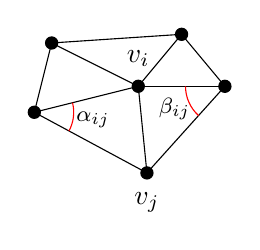
\begin{tikzpicture}[scale=1.1]
    \coordinate (i) at (0,0);
    \coordinate (A) at (1,0);
    \coordinate (B) at (0.5,0.6);
    \coordinate (C) at (-1,0.5);
    \coordinate (D) at (-1.2,-0.3);
    \coordinate (E) at (0.1,-1);

    \node[label=below:{$v_j$}] (EN) at (E) {};
    \node[label=above:{$v_i$}] (iN) at (i) {};

    \draw (i) -- (A);
    \draw (i) -- (B);
    \draw (i) -- (C);
    \draw (i) -- (D);
    \draw (i) -- (E);

    \draw (A) -- (B);
    \draw (B) -- (C);
    \draw (C) -- (D);
    \draw (D) -- (E);
    \draw (E) -- (A);

    \pic [draw=red, -, "\footnotesize{$\alpha_{ij}$}", angle eccentricity=1.5] {angle = E--D--i};
    \pic [draw=red, -, "\footnotesize{$\beta_{ij}$}", angle eccentricity=1.4] {angle = i--A--E};
       
      
    \draw[fill=black, draw=black] (i) circle (2pt);
    \draw[fill=black, draw=black] (A) circle (2pt);
    \draw[fill=black, draw=black] (B) circle (2pt);
    \draw[fill=black, draw=black] (C) circle (2pt);
    \draw[fill=black, draw=black] (D) circle (2pt);
    \draw[fill=black, draw=black] (E) circle (2pt);
\end{tikzpicture}

    (b) \includegraphics[width=.4\linewidth]{figures/projection.png}
    \caption{Discretization of the Laplace Beltrami operator on a mesh (a) and a point cloud (b). In the mesh the connectivity is directly given and can be used to compute properties like angles. The point cloud Laplacian relies on a approximation of tangent plane at a point on which the neighborhood is projected (blue). }
    \label{fig:cotan}
\end{figure}

The cotan-discretization \cite{pinkallporthier} for triangular meshes is defined as follows:
\begin{align}
    W_{ij} = \begin{cases}
        \frac{1}{2} (\text{cot}\alpha_{ij} + \text{cot} \beta_{ij}), & \text{if } (i,j) \in E \\
        - \sum_{k \in \mathcal{N}(i)} w_{ik}, & \text{if } j=i \\
        0, & \text{otherwise}
    \end{cases}
\end{align}
where $\alpha_{ij}, \beta_{ij}$ are the opposing angles to the edge between vertices $v_i, v_j$ (see \cref{fig:cotan}). 
In combination with the diagonal mass matrix $M$ describing the local weight at each vertex $M_{ii}$ the area of the voronoi cell around vertex $i$, the LBO is $L = M^{-1} W$.
While the default cotan-Laplacian does not fulfill the maximum principle, it will when applied to the intrinsic Delaunay triangulation of the input mesh \cite{bobenko2007simplicial}.
However, this depends on a clean mesh with only triangles and no non-manifoldness (e.g., edges with three triangles attached). 
For meshes of arbitrary topology, \cite{sharp2020nonmanifold} suggested to use the tufted cover, which generates an implicit manifold overlay of a given connectivity, in combination with the intrinsic triangulation. 
Due to its flexibility w.r.t. the connectivity, the tufted Laplacian is also well-suited to be used on point clouds by approximating a local neighborhood and connectivity for each point without the need to reconstruct a full, consistent triangle mesh, which is expensive and prone to be noisy. 

% introduce PDDL domains
% why Gripper env as testing context
% motivation: comparing classical vs LLM planners
% - classical: PDDL solver fast-downward
% - LLM: gpt-4o
% explanation and refinement are two distinguishing features of LLM planners
% - how we demonstrate explanation and refinement in the study
We evaluate user trust in two planners over a set of planning problems and study the potential factors influencing user trust in the planners. In particular, we compare a language-model-based planner, denoted as an \emph{LLM Planner}, with a traditional graph-search-based planner, denoted as a \emph{PDDL Solver}. The PDDL Solver uses Fast Downwards \cite{fastdownward} as its underlying model, processing planning problems described in PDDL to generate an optimal solution. In comparison, the LLM Planner employs GPT-4o to interpret the planning problem and extract a solution generated by the language model. Unlike the PDDL Solver, the LLM Planner can reason through the planning problem, explain its proposed solution, and iteratively refine the solution based on external feedback. This study investigates how the correctness of solutions, the quality of explanations, and the refinement process influence user trust.

\subsection{Planning Problem}
% \begin{wrapfigure}{r}{0.4\textwidth}
% % \begin{figure}[t]
%     \centering
%     \includegraphics[width=\linewidth]{figures/problem-example.pdf}
%     \caption{A running example of a planning problem in our study.}
%     \Description{Planning Problem Example}
%     \label{fig: problem-example}
% % \end{figure}
% \end{wrapfigure}

We describe each planning problem in the \emph{Planning Domain Definition Language (PDDL)} and propose two planners to generate plans that solve the problem. We select the \emph{gripper} planning problems from the International Planning Competition \cite{IPC} for plan generation and evaluation. In a gripper planning problem, a robot moves balls between a set of rooms using two grippers. The objective is to create a plan for the robot to move the balls to the target rooms we defined. We present a few running examples of the gripper problem in Figure \ref{fig: correctness}.

A planning problem consists of a \emph{planning domain} and a \emph{problem description}, expressed in PDDL. 

\paragraph{Planning Domain}
A planning domain refers to the universal aspects of a problem that remains consistent across different instances of the problem. In particular, it defines the types of objects, predicates, and actions that exist in the planning problem. We present an example of the gripper problem in Appendix \ref{app: grippers}.

\paragraph{Problem Description} A problem description specifies the particular instance of a planning task within a given domain. It includes the planning domain to which it pertains, a set of objects, the initial state of these objects, and the goal state to be achieved.

\paragraph{Plan}
A plan is a sequence of actions with specific input parameters. Recall that an action corresponds to a state transition. If a plan (a sequence of actions) transits from the initial state to the goal state defined by a problem, then we consider the plan to be \emph{correct}. If a plan does not transit to the goal state or there exists an action violating its precondition, then the plan is \emph{wrong}.

\begin{figure}[t]
    \centering
    \includegraphics[width=0.8\linewidth]{figures/correct.jpeg}
    \caption{Examples where LLM Planner correctly generates a plan for the gripper planning problem.}
    \Description{Planning Problem Correctness}
    \label{fig: correct}
\end{figure}

\subsection{PDDL Solver}
The PDDL Solver takes the planning domain and the problem description as inputs and then generates a plan described in PDDL. 
% It generates a plan in the following format:
% \vspace{4pt}
% \begin{lstlisting}[language=completion]
% (move robot1 room1 room3)
% (pick robot1 ball2 room3 rgripper1)
% (move robot1 room3 room2) ......
% \end{lstlisting}
Next, we convert the generated plan into natural language for user studies following the procedure in \cite{seipp-et-al-zenodo2022} and display it to users. We present an example in Figure \ref{fig: correct}.

The PDDL Solver applies a graph search algorithm to find a path (i.e., a list of transitions) from the initial state to the goal state. It either generates a \emph{correct} plan---defined as the shortest path between the initial and goal states---or returns a signal indicating that no solution exists for the given problem.

\subsection{LLM Planner}

The LLM Planner addresses planning problems by querying a large language model. In particular, it transmits the planning domain and problem description to the language model using a structured prompt format. The planner then retrieves a natural language plan from the language model. We use GPT-4o as the language model for the planner. To ensure the output adheres to the desired format, we include a few in-context examples within the prompts.

A language model solves a planning problem by interpreting the domain and problem descriptions, simulating state transitions, and generating a sequence of actions to achieve the goal. While effective for reasoning and plan generation, language models may struggle with large state spaces. Unlike the PDDL Solver, the LLM Planner may generate \emph{incorrect} plans that violate the problem specifications (e.g., preconditions of actions) or fail to achieve the goal.

\subsection{Explanation and Refinement}
Alongside the generated plans, we offer detailed explanations of all the plans and revisions of any incorrect plans. This study examines how these explanations and refinements influence human trust in the two planners.

\paragraph{LLM Planner with Explanation (LLM+Expl)}
For each generated plan, we manually provide a natural language explanation. This explanation includes an assessment of the plan’s correctness, identification of any violations of action preconditions, and an analysis of inconsistencies between the final state achieved and the intended goal state. We present examples of explanations in Figure \ref{fig: explain} in Appendix.

In particular, if a plan is correct, the explanation is simply ``the plan successfully satisfies the goal conditions.'' 
If a plan is incorrect, we identify the underlying cause as either a violation of action preconditions or a failure to achieve the goal state. In cases involving precondition violations, we specify the action responsible for the issue. For example, consider the action ``robot moves from room 1 to room 2,'' but the robot is initially located in room 3. This scenario constitutes a violation of the precondition for the ``move'' action. In the latter case, we describe the differences between the final state achieved and the intended goal state, e.g., ``fail to move ball 2 to room 2.''

% \begin{wrapfigure}{r}{0.5\textwidth}
%     \centering
%     \includegraphics[width=0.98\linewidth]{figures/refine.jpeg}
%     \includegraphics[width=0.98\linewidth]{figures/refine-correct.jpeg}
%     \includegraphics[width=0.98\linewidth]{figures/refine-wrong.jpeg}
%     \caption{Plan refinement by the LLM Planner. The top row presents two choices of plan refinement (where the refinement starts). The second and third row shows the refinement outcomes of the two choices, where the second row shows a correctly refined plan and the third row shows an incorrect plan.}
%     \Description{Refinement}
%     \label{fig: refine}
% \end{wrapfigure}

\paragraph{LLM Planner with Refinement (LLM+Refine)}
Note that a plan generated by the LLM Planner could be incorrect. Therefore, we offer a prompting mechanism for the LLM Planner to refine the generated plan according to the user feedback. The mechanism works as follows:

1. Request the user to indicate the step number of the first action in the plan that is incorrect, such as the step where an action’s precondition is violated. We present a sample user interface on the left of Figure \ref{fig: refine} in Appendix.

2. Send the planning domain, problem description, and the original plan to the language model. Then, query the model to rewrite the subsequent steps starting from the user-specified step number. We present a sample input prompt in Figure \ref{fig: refine-prompt} in the Appendix.

3. Replace the original plan with the newly refined plan and display it to the user.

This mechanism allows users to interact with the language model to refine the plan. It enables the language model to focus on a subset of steps, facilitating a deeper interpretation of the incorrect component. However, the correctness of the refined plan is not guaranteed. Figure \ref{fig: refine} in the Appendix shows an example of a correctly refined plan and an incorrectly refined plan.

\section{Experiments}
\label{sec:experiments}

\begin{figure*}[t]
\vspace{-6mm}
    \centering
    \includegraphics[width=0.8\linewidth]{figs/compare.pdf}
    \vspace{-4mm}
    \caption{\textbf{Qualitative comparison} with the baseline for generating a sequence of novel view images.  
    The results demonstrate that our method synthesizes more consistent multi-view images compared to our baseline model (Zero123). In addition, compared to SyncDreamer, our method visually maintains better similarity to the conditioned image and appears more natural.}
    \label{fig:sota_compare}
\vspace{-5mm}
\end{figure*}

\subsection{Experimental Setups}
\textbf{Dataset.}
Following previous work~\cite{zero123, SyncDreamer}, we evaluate our work on the Google Scanned Object (GSO)~\cite{GSO} dataset to verify the zero-shot novel view image synthesis capability. 
We also provide results for additional datasets in the Supplementary Material.
Specifically, we randomly select 30 objects from the GSO dataset with various object categories. 
Unlike recent approaches~\cite{mvdream, SyncDreamer} that aim to enhance the consistency of novel view synthesis models by generating multiple fixed-view images, our method can generate images from any camera pose and any number of views. Therefore, we conduct experiments under different camera pose settings to validate our approach:
specifically, 
1) \textit{16-views with free camera pose}: for each object, we circularly render 16 views with the elevation angles ranging in $[-10\degree, 40\degree]$ and the azimuth angles are evenly distributed in $[0\degree, 360\degree]$. 
2) \textit{16-views with fixed camera pose}: We maintain a constant elevation angle of $30\degree$ and uniformly sample azimuth angles (same as SyncDreamer~\cite{SyncDreamer}).
3) \textit{32-views with free camera pose}: Similar to the first setting, but we sample 32 views.
It's important to note that our method does not require additional training or fine-tuning on any datasets.

\noindent\textbf{Metrics.}
To validate the effectiveness of our method, we mainly evaluate it based on three criteria:
1) \textit{Quality Score}. We evaluate the image quality of synthesized multi-view images by measuring their similarity with ground truth images. Following prior research~\cite{zero123, sparsefusion}, we report the similarity between the synthesized images and the ground truth images with standard metrics: PSNR, SSIM~\cite{ssim}, and LPIPS~\cite{lpips}.
2) \textit{Multi-view Consistency Score}. As the primary goal of our work is to improve the consistency of generated images, we also employ the 3D consistency score~\cite{3dim} to verify the consistency among the synthesized images. Specifically, we train an Instant-NGP~\cite{instant_ngp} with the input image and part of the synthesized novel view images of our model and evaluate the similarity between the remaining synthesized images and the rendered images of Instant-NGP. For the synthesized multi-view images of each object, we allocate $3/4$ for training and reserve the remaining $1/4$ for validation.
Intuitively, if the consistency of synthesized images is improved, the NeRF-like model will train a better object representation, and the re-rendered images will agree more with the validation images.
3) \textit{Input Consistency Score}. To assess the faithfulness of synthesized images in preserving the identity of the input condition image, we introduce the input consistency score. This score calculates the similarity of each synthesized image with the input condition image, utilizing the LPIPS metric.

In addition, we use synthesized multi-view images to train a neural 3D reconstruction model (NeuS~\cite{neus}) and report commonly used Chamfer Distances (CD) and Volume IoUs between the trained 3D model and the ground truth.

\noindent\textbf{Baselines.}
Given that our main goal is to improve the consistency of the trained baseline model without further fine-tuning, we mainly compare our approach with the used baseline model Zero123~\cite{zero123}. Additionally, we compare our method to the SOTA approaches such as PGD~\cite{tseng2023consistent} and SyncDreamer~\cite{SyncDreamer} using the same Zero123 base model.

\noindent\textbf{Implementation Details.}
We use the official checkpoint provided by Zero123~\cite{zero123}, which is trained on objaverse~\cite{objaverse} for 165,000 steps. We inject our epipolar attention layer after step $T=4$ and layer $L=10$ by default. We find that feature fusion weight $\alpha=0.5$, and the number of context views $M=2$ work better.

\begin{table}[t]
\centering
\caption{Comparison of multi-view consistency, image quality, and input consistency of synthesized multi-view images at the 16-view setting with free camera pose.}
\label{tab:view16_free_compare}
\vspace{-2mm}
\scalebox{0.6}{
\begin{tabular}{c ccc ccc c}
\toprule
              & \multicolumn{3}{c}{Multi-view Consistency} & \multicolumn{3}{c}{Quality Score} & \multicolumn{1}{c}{Input Consis.} \\
              \cmidrule(lr){2-4} \cmidrule(lr){5-7} \cmidrule(lr){8-8}
              & PSNR$\uparrow$  & SSIM$\uparrow$ & LPIPS$\downarrow$ 
              & PSNR$\uparrow$  & SSIM$\uparrow$ & LPIPS$\downarrow$ 
              & LPIPS$\downarrow$ 
              \\ \midrule

Zero123
& 15.225        & 0.645       & 0.408
& 14.255        & 0.747       &	0.208
& 0.303         
\\
SyncDreamer
& 14.830        & 0.626       & 0.434
& 12.650        & 0.713       &	0.254
& 0.317         
\\
Ours 
& \best{18.300}	& \best{0.734}	& \best{0.355}
& \best{14.947}	& \best{0.763}	& \best{0.191}
& \best{0.282}
\\

\bottomrule
\end{tabular}
}
\end{table}

\begin{table}[t]
\vspace{-1mm}
\centering
\caption{Comparison of multi-view consistency, image quality, and input consistency at the 16-view setting with fixed camera pose as SyncDreamer~\cite{SyncDreamer}.}
\label{tab:view16_fxied_compare}
\vspace{-3mm}
\scalebox{0.6}{
\begin{tabular}{c ccc ccc c}
\toprule
              & \multicolumn{3}{c}{Multi-view Consistency} & \multicolumn{3}{c}{Quality Score} & \multicolumn{1}{c}{Input Consis.} \\
              \cmidrule(lr){2-4} \cmidrule(lr){5-7} \cmidrule(lr){8-8}
              & PSNR$\uparrow$  & SSIM$\uparrow$ & LPIPS$\downarrow$ 
              & PSNR$\uparrow$  & SSIM$\uparrow$ & LPIPS$\downarrow$ 
              & LPIPS$\downarrow$ 
              \\ \midrule

Zero123
& 16.556        & 0.682       & 0.378
& 14.592        & 0.750       &	0.207
& 0.305         
\\
SyncDreamer
& \best{22.424}        & \best{0.812}       & \best{0.268}
& 15.269        & 0.749       &	0.196
& 0.300         
\\
Ours 
& 21.151	& 0.780	& 0.302
& \best{15.293}	& \best{0.764}	& \best{0.184}
& \best{0.287}
\\

\bottomrule
\end{tabular}
}
\vspace{-4mm}
\end{table}


\subsection{Comparison With Baseline Models}
The quantitative comparison on three settings are shown in Tab.~\ref{tab:view16_free_compare}, Tab.~\ref{tab:view16_fxied_compare}, and Tab.~\ref{tab:view32_free_compare}. The qualitative comparison is shown in Fig.~\ref{fig:sota_compare}.

\begin{table}[t]
\centering
\caption{Comparison of multi-view consistency and image quality scores of synthesized multi-view images at the 32-view setting with free camera pose.}
\vspace{-3mm}
\label{tab:view32_free_compare}
\scalebox{0.7}{
\begin{tabular}{c ccc ccc}
\toprule
              & \multicolumn{3}{c}{Multi-view Consistency} & \multicolumn{3}{c}{Quality Score} \\
              \cmidrule(lr){2-4} \cmidrule(lr){5-7}
              & PSNR$\uparrow$  & SSIM$\uparrow$ & LPIPS$\downarrow$ 
              & PSNR$\uparrow$  & SSIM$\uparrow$ & LPIPS$\downarrow$ 
              \\ \midrule

Zero123
& 16.515        & 0.694       & 0.378
& 15.142        & 0.733       &	0.211
\\
PGD~\cite{tseng2023consistent}
& 18.481        & 0.720       & 0.343
& 15.281        & 0.739       &	0.205
\\
Ours 
& \best{20.655}	& \best{0.792}	& \best{0.305}
& \best{15.268}	& \best{0.742}	& \best{0.203}
\\

\bottomrule
\end{tabular}
}
\vspace{-3mm}
\end{table}

\begin{table*}
  [t]
  \centering
  \resizebox{\textwidth}{!}{%
  \begin{tabular}{cccccccccccc}
    \toprule \multicolumn{2}{c}{Components}                                                             & \multicolumn{5}{c}{Re-executability Rate (\%)} & \multicolumn{5}{c}{Readability (\#)} \\
    \cmidrule(lr){1-2} \cmidrule(lr){3-7} \cmidrule(lr){8-12}        \hspace{8pt}\labelemoji\hspace{8pt}                                                                & \hspace{8pt}\toolemoji\hspace{8pt}                                      & O0                                 & O1             & O2             & O3             & AVG            & O0             & O1             & O2             & O3             & AVG            \\
    \hline
    \rowcolor[rgb]{0.93,0.93,0.93}\multicolumn{12}{c}{\textbf{Initialize with LLM4Decompile-End-6.7B~\citep{llm4decompile}}}   \\
    \xmark                                                                                              & \xmark                                    & 69.51                              & 46.95          & 50.61          & 46.34          & 53.35          & 3.98 & 3.41 & 3.44 & 3.38 & 3.55 \\
    \cmark                                                                                              & \xmark                                    & 75.61                              & 50.61          & 50.00          & 50.00          & 56.55          & 4.01 & 3.44 & 3.39 & \textbf{3.49} & 3.58 \\
    \xmark                                                                                              & \cmark                                    & 83.54                     & \textbf{56.10}          & 51.22          & 50.61 & 60.37 & 4.05 & 3.51 & 3.51 & 3.42 & 3.62 \\
    \cmark                                                                                              & \cmark                                    & \textbf{85.37}                            & \textbf{56.10}                     & \textbf{51.83} & \textbf{52.43}          & \textbf{61.43} & \textbf{4.13} & \textbf{3.60} & \textbf{3.54} & \textbf{3.49} & \textbf{3.69} \\

    \rowcolor[rgb]{0.93,0.93,0.93}\multicolumn{12}{c}{\textbf{Initialize with Deepseek-Coder-6.7B-base~\citep{deepseekcoder}}} \\
    \xmark                                                                                              & \xmark                                    & 59.15                              & 35.98          & 39.02          & 37.80          & 42.99          & 3.71 & 3.05 & 3.16 & 3.05 & 3.24 \\
    \cmark                                                                                              & \xmark                                    & 66.46                              & 41.46          & 38.41          & 36.59          & 45.73          & 3.76 & 3.17 & \textbf{3.21} & 3.08 & 3.31 \\
    \xmark                                                                                              & \cmark                                    & 70.73                              & 39.63          & 39.02          & 40.24          & 47.41          & 3.90 & 3.17 & 3.08 & 3.11 & 3.31 \\
    \cmark                                                                                              & \cmark                                    & \textbf{79.88}                     & \textbf{45.73} & \textbf{43.90} & \textbf{42.68} & \textbf{53.05} & \textbf{3.96} & \textbf{3.21} & 3.18 & \textbf{3.19} & \textbf{3.38} \\
    \bottomrule
  \end{tabular}%
  }
  \caption{The ablation study of different methods across four optimization levels
  (O0, O1, O2, O3), as well as their average scores (AVG). The results in bold represent the optimal performance. The ~\labelemoji~ and ~\toolemoji~ means Relabedling and Function Call. \textbf{Bold} denotes the best performance.}
  \label{tab:ablation}
\end{table*}



\begin{figure*}[ht]
    \centering
    \begin{minipage}{0.65\textwidth}
        \centering
        \includegraphics[width=0.95\linewidth]{figs/ablation.pdf}
        \vspace{-2mm}
        \captionof{figure}{Qualitative Comparison for different design choices. Our method, employing multi-view epipolar attention, demonstrates the best consistency.}
        \label{fig:ablation}
    \end{minipage}\hfill
    \begin{minipage}{0.33\textwidth}
        \centering
        \includegraphics[width=0.8\linewidth]{figs/neus_ver.pdf}
        \vspace{-3mm}
        \caption{Our method shows better direct 3D reconstruction~\cite{neus}.}
        \label{fig:neus}
    \end{minipage}
    \vspace{-5mm}
\end{figure*}

\noindent\textbf{Multi-view Consistency.}
Tab.~\ref{tab:view16_fxied_compare} presents the 3D consistency scores compared to our baseline model (Zero123) and SyncDreamer. The results indicate a significant improvement across all three metrics achieved by our method when compared with Zero123.
While our method exhibits a marginally lower numerical consistency score compared to SyncDreamer, it enables the synthesis of images with arbitrary camera poses.	
This capability is illustrated in Tab.~\ref{tab:view16_free_compare}, where our method consistently enhances consistency with changes in camera pose settings, whereas SyncDreamer fails to do so and exhibits inferior results compared to Zero123.
Furthermore, our method facilitates the synthesis of multi-view images with any number of camera views. This versatility is demonstrated in Tab.~\ref{tab:view32_free_compare}, where our method continues to achieve significant improvements in consistency scores, while SyncDreamer is unable to operate under such conditions.	

Meanwhile, Fig.~\ref{fig:sota_compare} provides a qualitative comparison with the baseline. While both our method and SyncDreamer enhance consistency, our method visually preserves better similarity to the input image, including color and texture details. The input consistency score further corroborates this.

\noindent\textbf{Image Quality.}
While our primary goal centers around enhancing the consistency of synthesized multi-view images, we also evaluate the image quality by comparing the similarity with the ground truth images. The results shown in Tab.~\ref{tab:view16_free_compare}, Tab.~\ref{tab:view16_fxied_compare}, and Tab.~\ref{tab:view32_free_compare} indicate that our method also enhances the image quality under different settings besides improving the consistency.
Moreover, our method shows better image quality compared with SyncDreamer even in the 16-view setting with fixed camera pose.

\noindent\textbf{Input Consistency.}
Input consistency terms whether the results align with the input image.
Fig.~\ref{fig:sota_compare} illustrates that both our method and SyncDreamer enhance multi-view consistency. However, the color and texture details of SyncDreamer's results diverge from the input image and appear visually unnatural.
This discrepancy is evident in the input consistency score presented in Tab.~\ref{tab:view16_fxied_compare}, indicating lower similarity with the condition image in the SyncDreamer results.	

\subsection{Ablation Study}
The overall quantitative results are shown in Tab.~\ref{tab:ablation}, and the qualitative comparisons are shown in Fig.~\ref{fig:ablation}.

\noindent \textbf{Full Attention \vs Epipolar Attention.}
The results presented in Tab.\ref{tab:ablation} and Fig.\ref{fig:ablation} demonstrate that our epipolar attention mechanism can synthesize more consistent multi-view images compared with full attention. Furthermore, our epipolar attention achieves a greater performance improvement compared to full attention when using multiple reference images. This could be attributed to the fact that our epipolar attention more effectively localizes target information, as depicted in Fig.~\ref{fig:full_attn_compare}, thereby reducing noise from the reference images. In the multi-view setting, where multiple reference images are utilized, this noise reduction becomes particularly crucial.
Moreover, it is noteworthy that the epipolar attention mechanism consumes less GPU memory compared to our baseline, as discussed in Sec.~\ref{sec:attn_analysis}.

\noindent \textbf{Attending Single-View \vs Multi-View.}
Applying the epipolar attention significantly improves the consistency between the input and target views. However, the consistency between different views in the unobserved regions of the input view is not well preserved.
After implementing our epipolar attention in the multi-view setting, the consistency across the generated multi-view images is further improved. The last row in Tab.~\ref{tab:ablation} shows that after applying our multi-view epipolar attention, the consistency score is further improved compared with the single-view setting. Besides, the qualitative result in Fig.~\ref{fig:ablation} also shows better consistency among different target views.



\begin{table}[t]
\centering
\vspace{-1mm}
\caption{Comparison of 3D reconstruction results. Our method significantly improves the reconstruction quality.}
\vspace{-3mm}
\label{tab:neus}
\scalebox{0.7}{
\begin{tabular}{c cc}
\toprule
              &  Chamfer Dist.$\downarrow$  & Volume IoU$\uparrow$
\\ \midrule

            Zero123         & 0.017         & 0.819    \\
            SyncDreamer     & \best{0.013}         & \best{0.847}    \\
            Ours            & 0.014	& 0.842 \\

\bottomrule
\end{tabular}
}
\vspace{-5mm}
\end{table}


\vspace{-2mm}
\subsection{Downstream Application}
\vspace{-2mm}
To demonstrate the effectiveness of our method, we also applied it to the downstream 3D reconstruction task. Specifically, we trained the NeuS model~\cite{neus} directly using images synthesized by our method, Zero123, and SyncDreamer, respectively.
The quantitative results in Tab.~\ref{tab:neus} show that the consistent multi-view images synthesized by our method can significantly improve the 3D reconstruction quality.
Additionally, our method exhibits similar performance to SyncDreamer which requires time-consuming re-training.
The qualitative results in Fig.~\ref{fig:neus} show that it is challenging to train the NeuS model directly due to the lack of consistency in the images generated by Zero123. In contrast, our method generates more consistent multi-view images and, therefore, better reconstructs the geometry and texture details.
We show improvements on other downstream applications such as image-to-3D in the Supplementary Material.


\section{Conclusion}

%In this paper, w
We propose a new PEFT method called DiffoRA, which enables efficient and adaptive LLM fine-tuning based on LoRA. 
Instead of adjusting every interior rank, 
%of the decomposition matrices 
%of all modules, 
we argue that adopting LoRA module-wisely is sufficient. 
To achieve this, we construct a DAM to select the modules that are most suitable and essential to fine-tune. We theoretically analyze how the DAM impacts the convergence rate and generalization capability.
%of the pre-trained model. 
Furthermore, we adopt continuous relaxation and discretization to establish DAM.
%for each task. 
To alleviate the issue of discretization discrepancy, we utilize the weight-sharing strategy for optimization. 
%We fully implement our method and t
The experimental results demonstrate that our DiffoRA works consistently better than the baselines across all benchmarks. 
{
    \small
    \bibliographystyle{ieeenat_fullname}
    \bibliography{main}
}


\end{document}
